\chapter{Analyse et spécification des besoins}

Le contexte posé, restait à traduire la problématique en besoins concrets : qui utilise la plateforme, pour faire quoi, et avec quelles contraintes ? C’est ce que je détaille dans ce chapitre, acteur par acteur, avant de justifier les choix techniques préliminaires qui ont guidé l’architecture retenue.

\section{Introduction}
\label{sec_2_1}
Recueillir les besoins n’a rien eu d’un exercice ponctuel : cela s’est étalé sur les premières semaines du stage, au fil des échanges avec mon encadrant et de l’observation directe du processus RH. Ce qui suit est le résultat de cette phase, et sert de base directe à la conception présentée au chapitre suivant.

\section{Étude fonctionnelle}
\label{sec_2_2}
\subsection{Identification des acteurs du système}
\label{sec_2_2_1}
Cinq acteurs interviennent sur la plateforme JOB4YOU, chacun avec ses propres privilèges et fonctionnalités :

\begin{itemize}
\item Le Visiteur : utilisateur anonyme, non authentifié, qui consulte les offres d’emploi publiées et peut déposer son CV dans la fonctionnalité « Job idéal » pour obtenir des suggestions ; il doit créer un compte et s’authentifier pour soumettre une candidature.
\item Le Candidat : utilisateur authentifié disposant d’un compte (rôle ROLE\_USER), qui soumet ses candidatures, en suit l’avancement, échange avec l’assistant conversationnel et peut retirer un dossier tant qu’il n’est pas clos.
\item Le Responsable RH : acteur central du processus, il publie les offres, examine et valide les candidatures, planifie les entretiens et contresigne la décision finale (embauche ou refus), seul moment où le candidat est notifié.
\item Le Manager : intervient à partir de l’entrée du dossier en évaluation technique (statut TECHNICAL\_TEST) ; il consulte les candidatures relevant de son périmètre, mène ou participe aux entretiens, fournit un feedback structuré et émet un avis (favorable ou refus proposé) sur les dossiers de son périmètre, qui reste à contresigner par le RH.
\item L’Administrateur : acteur transverse chargé de la gestion des comptes utilisateurs, des rôles, du paramétrage du scoring IA par famille de métier et de la supervision globale de la plateforme (journal d’audit).
\end{itemize}

Le tableau~\ref{tab_2_1} précise, action par action, les rôles habilités — une répartition qui correspond exactement aux règles d’autorisation implémentées côté back-end.

% tableau 2.1
\setcounter{table}{0}
\begin{table}[!ht]
\centering
\caption{Matrice des responsabilités par rôle}
\label{tab_2_1}
\renewcommand{\arraystretch}{1.25}\footnotesize
\setlength{\tabcolsep}{4pt}%
\begin{tabular}{|P{0.441\textwidth}|P{0.093\textwidth}|P{0.164\textwidth}|P{0.121\textwidth}|P{0.093\textwidth}|}
\hline
\textbf{Action} & \textbf{RH} & \textbf{Manager} & \textbf{Administrateur} & \textbf{Candidat} \\
\hline
Publier / gérer une offre d’emploi & Oui & Non & Oui & Non \\
\hline
Valider un CV (passage CV\_REVIEWED) & Oui & Non & Oui & Non \\
\hline
Planifier un entretien & Oui & Oui (son périmètre) & Oui & Non \\
\hline
Saisir un feedback & Oui & Oui & Oui & Non \\
\hline
Valider / transmettre un feedback au candidat & Oui & Non & Oui & Non \\
\hline
Avis sur la candidature (favorable / refus proposé) & Oui & Oui (son périmètre) & Oui & Non \\
\hline
Décision finale contresignée (HIRED / REJECTED) & Oui & Non & Oui & Non \\
\hline
Gérer les utilisateurs et les rôles & Non & Non & Oui & Non \\
\hline
Paramétrer le scoring IA & Non & Non & Oui & Non \\
\hline
Consulter le journal d’audit & Oui & Non & Oui & Non \\
\hline
\end{tabular}
\end{table}
J’ai volontairement donné au RH et à l’Administrateur la main sur l’ensemble du cycle : ils peuvent enregistrer un avis comme le ferait le manager — pour corriger ou débloquer un dossier en son absence — et sont seuls à pouvoir contresigner la décision finale. Un compte purement manager ne peut écrire ni l’embauche (HIRED) ni un statut du pipeline : la plateforme le refuse par une erreur 403. Qui a réellement pris chaque décision reste visible dans le journal d’audit.

\subsection{Identification des besoins fonctionnels}
\label{sec_2_2_2}
Les échanges avec mon encadrant entreprise et l’étude de l’existant ont fait émerger les besoins fonctionnels suivants :

\begin{itemize}
\item Authentification et gestion des sessions sécurisée par jeton JWT, avec gestion différenciée des accès selon le rôle de l’utilisateur.
\item Gestion des offres d’emploi : création, modification, publication, clôture et expiration automatique des offres dont la date limite est dépassée.
\item Gestion des candidatures : soumission en ligne avec dépôt de CV, consultation, filtrage et suivi de l’état d’avancement de chaque dossier.
\item Analyse automatique des candidatures par intelligence artificielle : extraction du contenu du CV et calcul d’un score de pertinence (technique, communication, adéquation séniorité) avec possibilité de correction manuelle par le RH.
\item Gestion des entretiens : planification, changement de statut (planifié, en cours, terminé, annulé, reprogrammé), envoi d’invitations et de rappels automatiques.
\item Gestion des feedbacks : saisie d’un retour structuré par le manager après entretien, validation par le RH et notification au candidat.
\item Décision à deux niveaux : le manager émet un avis (favorable ou refus proposé) que le RH ou l’Administrateur contresigne pour produire la décision finale — embauche avec date de présentation des documents, ou refus motivé —, avec garde-fou empêchant toute décision sur un dossier non validé par le RH et toute validation finale par un compte purement manager.
\item Notifications automatiques par e-mail à chaque étape clé du processus (confirmation de candidature, invitation à un entretien, décision finale) ; l’e-mail de décision finale n’est adressé au candidat qu’après le contreseing du RH, l’avis du manager notifiant le RH ; seule exception, le refus prononcé par l’agent IA, notifié dès le statut AUTO\_REJECTED et qui n’est pas doublé lorsque le RH se borne à le confirmer.
\item Tableau de pilotage visuel de type Kanban permettant de visualiser en un coup d’œil la répartition des candidatures par statut.
\item Gestion des utilisateurs, des rôles et paramétrage des profils de pondération du score IA par famille de métier.
\item Matching inverse (« Job idéal ») : un visiteur peut déposer son CV sans postuler à une offre précise ; le système le compare aux offres actives et lui suggère les plus pertinentes avec un score de compatibilité.
\end{itemize}

\subsection{Identification des besoins non fonctionnels}
\label{sec_2_2_3}
Au-delà des fonctionnalités métier, la plateforme doit aussi répondre aux exigences non fonctionnelles suivantes :

\begin{itemize}
\item Sécurité : authentification robuste par jeton JWT signé d’une durée de vie de 24 heures, hachage des mots de passe avec BCrypt, contrôle d’accès basé sur les rôles (RBAC) appliqué à la fois côté front-end et côté back-end, jeton de réinitialisation de mot de passe valable 15 minutes et limitation du nombre de tentatives de connexion.
\item Performance : temps de réponse cible inférieur à 500 ms pour les opérations de lecture courantes et inférieur à 2 s pour les opérations d’écriture, chargement asynchrone des traitements longs (scoring IA, envoi d’e-mails) afin de ne pas bloquer l’utilisateur, et taille maximale des CV déposés fixée à 10 Mo côté serveur (formats PDF, DOC, DOCX), le formulaire de candidature refusant déjà les fichiers de plus de 5 Mo. Cette différence de plafond est volontaire : la validation du formulaire est un confort offert à l’utilisateur, la limite serveur est la véritable barrière de sécurité, seule opposée à un client qui contournerait l’interface.
\item Ergonomie et responsive design : interface claire, intuitive et utilisable aussi bien sur poste de travail que sur tablette.
\item Fiabilité : garde-fous métier empêchant les transitions de statut incohérentes (ex. acceptation avant l’entretien téléphonique RH, validation finale sans avis manager en attente, embauche sans date de présentation des documents, entretien planifié sur un dossier clos).
\item Maintenabilité et évolutivité : architecture modulaire en couches, séparation claire entre front-end, back-end et automatisation, facilitant l’ajout de nouvelles fonctionnalités.
\item Traçabilité : journalisation des actions sensibles (changements de statut, corrections de score) dans un journal d’audit.
\end{itemize}

\subsection{Diagramme d’activité — Vue d’ensemble du processus de recrutement}
\label{sec_2_2_4}
Avant de détailler les fonctionnalités attendues, ce diagramme d’activité pose le flux métier global : il décrit l’enchaînement des activités du processus de recrutement, de la publication de l’offre jusqu’à la décision finale, ainsi que les acteurs qui les portent, indépendamment de toute considération technique.

Le diagramme d’activité, présenté en trois volets (figures~\ref{fig_2_1a}, \ref{fig_2_1b} et \ref{fig_2_1c}), rend explicite un point que le texte seul rendait moins visible : l’entretien téléphonique RH est un passage obligé avant toute évaluation technique (section~\ref{sec_4_5_8}), et la transmission au manager désigné par le RH (section~\ref{sec_3_5_4}) n’intervient qu’à ce moment-là, pas dès la validation du CV — conformément à la correction décrite en section~\ref{sec_4_5_5}. Le rejet automatique par l’IA n’y constitue pas une fin de parcours distincte : il rejoint, comme le contreseing du RH, l’étape commune de notification et de journalisation, et admet deux issues humaines distinctes, toutes deux portées par la transition « AUTO\_REJECTED » de la figure~\ref{fig_3_8} : le RH confirme le refus après examen, ou le conteste par un override justifié qui le réintègre dans le pipeline, à condition que la note corrigée atteigne le seuil de 60/100.

Le volet~\ref{fig_2_1a} couvre le dépôt de la candidature et la présélection automatisée ; le volet~\ref{fig_2_1b} prend le dossier en charge côté RH et manager, jusqu’à l’avis du manager ; le volet~\ref{fig_2_1c} termine le parcours par la décision finale du RH, sa journalisation et la notification du candidat. Ce découpage en trois volets a été imposé par la lisibilité à l’impression : la vue d’ensemble, en une seule figure, ne rendait plus qu’en 5,4 pt imprimés sous la contrainte de la page paysage, alors que ces trois figures s’affichent entre 8,7 et 12,8 pt.

% figure 2.1a / 2.1b / 2.1c
% La vue d'ensemble tenait dans une seule figure paysage (fig2_1.png,
% 2221x1383 px) : ramenee a 0,98\linewidth x 0,90\textheight en paysage, elle
% n'imprimait plus ses etiquettes qu'a 5,4 pt, sous le plancher de 8 pt retenu
% pour ce rapport. Elle est donc decompee en trois volets enchaunes, chacun
% rendu a sa propre echelle : 8,7 pt imprimes pour 2.1a (paysage, ratio 2,3),
% 12,8 pt pour 2.1b (portrait) et 10,2 pt pour 2.1c (portrait). Les numeros a
% suffixe alphabetique suivent le procede deja utilise pour 3.2a/3.2b et
% 4.15a/4.15b, ce qui ne decale aucune figure du chapitre.
\setcounter{figure}{0}
\begingroup\renewcommand{\thefigure}{2.1a}
\begin{landscape}
\pagestyle{lscape}
\begin{figure}[p]
\centering
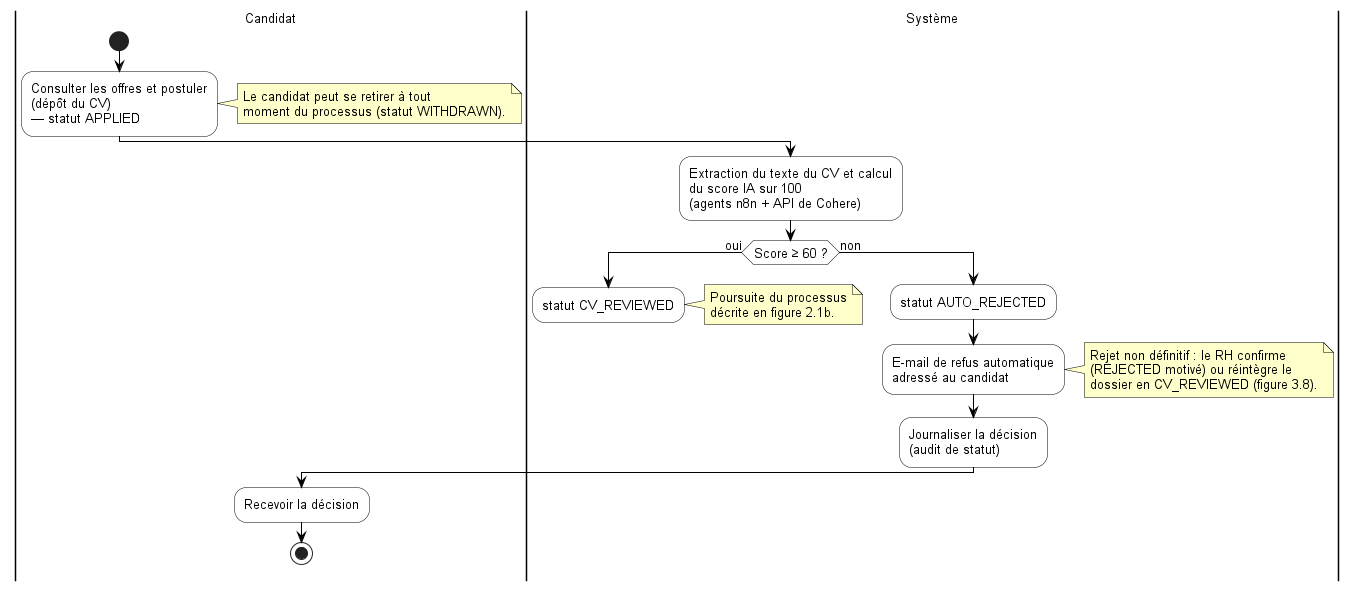
\includegraphics[width=0.98\linewidth, height=0.90\textheight, keepaspectratio]{fig2_1a}
\caption{Diagramme d’activité — Dépôt de la candidature et présélection automatisée par le score IA}
\label{fig_2_1a}
\end{figure}
\clearpage
\end{landscape}
\endgroup

\setcounter{figure}{0}
\begingroup\renewcommand{\thefigure}{2.1b}
\begin{figure}[!ht]
\centering
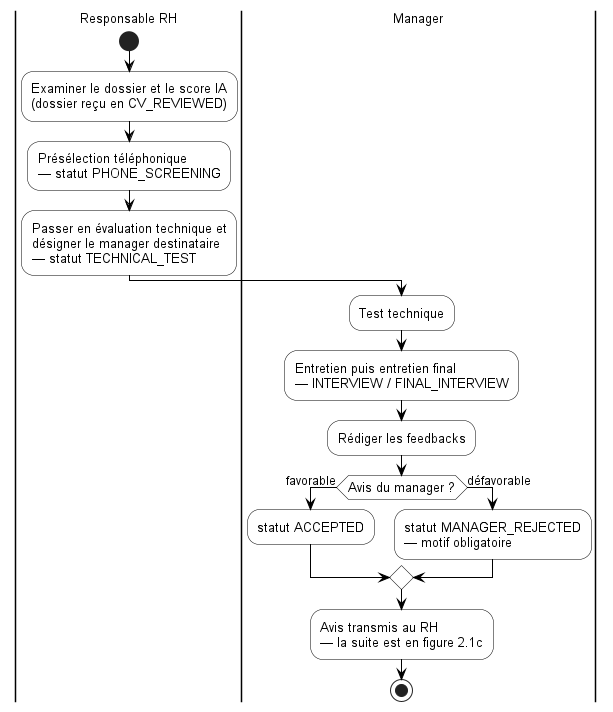
\includegraphics[width=0.98\linewidth, height=0.90\textheight, keepaspectratio]{fig2_1b}
\caption{Diagramme d’activité — Traitement du dossier par le RH et le manager, jusqu’à l’avis du manager}
\label{fig_2_1b}
\end{figure}
\endgroup

\setcounter{figure}{0}
\begingroup\renewcommand{\thefigure}{2.1c}
\begin{figure}[!ht]
\centering
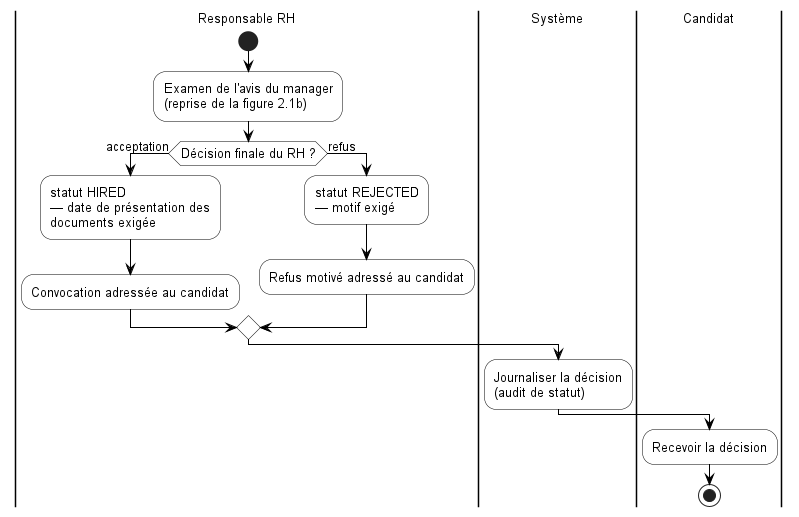
\includegraphics[width=0.98\linewidth, height=0.90\textheight, keepaspectratio]{fig2_1c}
\caption{Diagramme d’activité — Décision finale du RH, journalisation et notification du candidat}
\label{fig_2_1c}
\end{figure}
\endgroup

\subsection{Diagrammes de cas d’utilisation}
\label{sec_2_2_5}
Afin d’éviter l’effet « toile d’araignée », le périmètre fonctionnel est présenté en deux vues macro — l’espace public et candidat (figure~\ref{fig_2_2a}), puis les espaces réservés RH, manager et administrateur (figure~\ref{fig_2_2b}) — avant d’être décliné en trois sous-diagrammes par module (figures~\ref{fig_2_3} à \ref{fig_2_5}). Chaque vue est enfermée dans le cadre de la limite du système étudié, «~JOB4YOU~» : les acteurs restent à l’extérieur du cadre, les cas d’utilisation à l’intérieur, et les seules relations tracées relient soit un acteur à un cas (trait plein, sans flèche), soit un cas à un autre par «~include~» (pointillés, flèche pointée vers le cas inclus).

% figure 2_2
\setcounter{figure}{1}
\begingroup\renewcommand{\thefigure}{2.2a}
\begin{figure}[!ht]
\centering
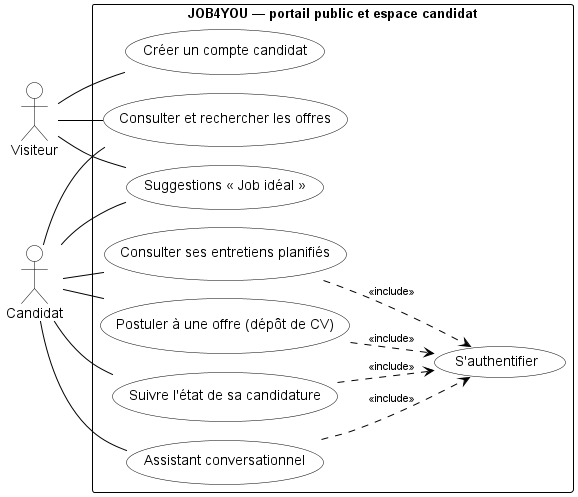
\includegraphics[width=0.98\linewidth, height=0.90\textheight, keepaspectratio]{fig2_2a}
\caption{Diagramme de cas d’utilisation global — espace public et candidat}
\label{fig_2_2a}
\end{figure}
\endgroup

% figure 2_2
\setcounter{figure}{1}
\begingroup\renewcommand{\thefigure}{2.2b}
\begin{figure}[!ht]
\centering
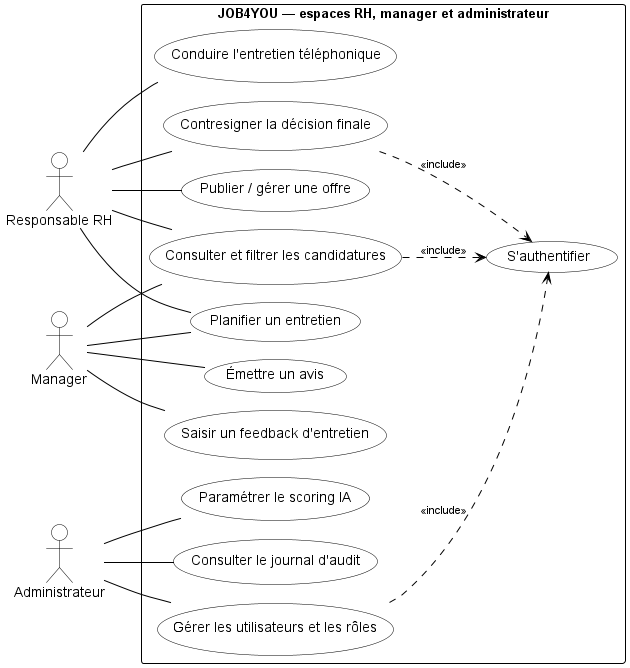
\includegraphics[width=0.98\linewidth, height=0.90\textheight, keepaspectratio]{fig2_2b}
\caption{Diagramme de cas d’utilisation global — espaces RH, manager et administrateur}
\label{fig_2_2b}
\end{figure}
\endgroup

L’authentification par jeton JWT est représentée par un cas unique « S’authentifier », auquel les cas des espaces sécurisés sont reliés par une relation « include ». Cette convention est celle du diagramme de cas d’utilisation global : elle est reprise ici sur sept cas représentatifs (postuler à une offre, suivre l’état de sa candidature, consulter ses entretiens planifiés, échanger avec l’assistant conversationnel, consulter et filtrer les candidatures, contresigner la décision finale, gérer les utilisateurs et les rôles) et s’applique en réalité à toutes les fonctionnalités des espaces sécurisés. Conformément à la norme UML \cite{ref03}, la flèche d’inclusion part du cas principal pour rejoindre le cas inclus ; aucune relation ne relie deux acteurs entre eux, ni deux cas hors de ce mécanisme. Le visiteur non authentifié conserve la consultation et la recherche des offres ainsi que les suggestions « Job idéal » ; le candidat authentifié reprend ces deux cas et y ajoute le dépôt de candidature, le suivi de son dossier, l’accès à ses entretiens et l’assistant conversationnel, qui lui est réservé. Les autorisations sont ensuite contrôlées côté serveur selon le rôle et le périmètre métier de l’utilisateur. Les diagrammes ne représentent que les cas principaux : la matrice du tableau~\ref{tab_2_1} fait foi pour le détail des droits. Certains droits y sont acceptés sans être retracés ici, pour ne pas transformer la figure en toile d’araignée : l’administrateur peut aussi publier une offre, planifier un entretien, émettre un avis et contresigner la décision finale ; le RH peut aussi saisir un feedback, émettre un avis et consulter le journal d’audit.
Le premier zoom couvre le portail public et candidat : consultation des offres, matching « Job idéal », dépôt de candidature et suivi en libre-service (figure~\ref{fig_2_3}).

% figure 2.3
\setcounter{figure}{2}
% le portrait a ete garde ici : ratio 1,25, le vrai paysage ne l agrandissait que de
% 13 % (544 pt contre 484 de large) tout en coutant une page pleine et la coupure
% du texte. En portrait l image imprime 8,2 pt, au-dessus de la cible de 8 pt.
\begin{figure}[!ht]
\centering
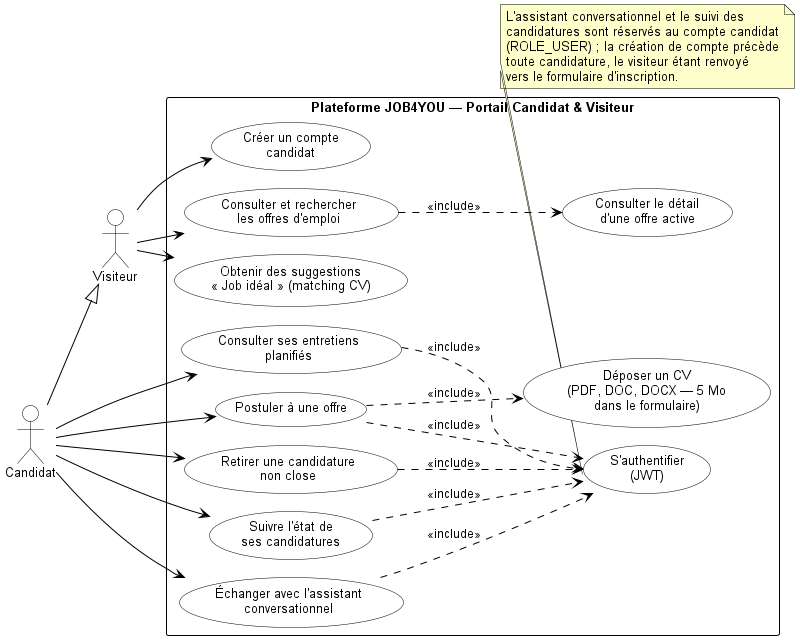
\includegraphics[width=\textwidth, height=0.80\textheight, keepaspectratio]{fig2_3}
\caption{Diagramme de cas d’utilisation — Portail Candidat \& Visiteur}
\label{fig_2_3}
\end{figure}

Le deuxième zoom décrit le cœur du processus côté RH et manager : publication des offres, filtrage, entretiens, feedbacks, avis du manager puis contreseing RH de la décision finale (figure~\ref{fig_2_4}). L’envoi des notifications par e-mail y est modélisé comme un cas inclus, déclenché par la planification ou par la décision, et non comme un cas autonome.

% figure 2.4
\setcounter{figure}{3}
\begin{figure}[!ht]
\centering
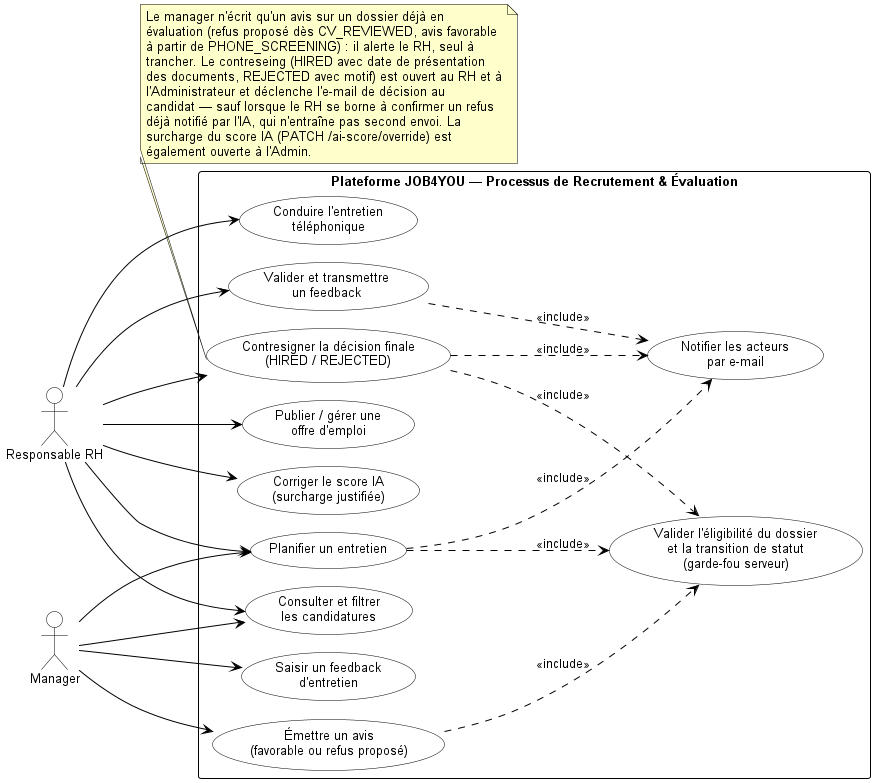
\includegraphics[width=\textwidth, height=0.80\textheight, keepaspectratio]{fig2_4}
\caption{Diagramme de cas d’utilisation — Processus de Recrutement \& Évaluation}
\label{fig_2_4}
\end{figure}

Le troisième zoom isole le périmètre d’administration : comptes et rôles, rattachement d’un utilisateur à un département ou à une famille de métier, pondérations du scoring IA et journal d’audit (figure~\ref{fig_2_5}). Le référentiel lui-même n’est pas administrable : les départements sont créés au démarrage et exposés en lecture seule, les familles de métier sont un énuméré figé dans le code.

% figure 2.5
\setcounter{figure}{4}
\begin{figure}[!ht]
\centering
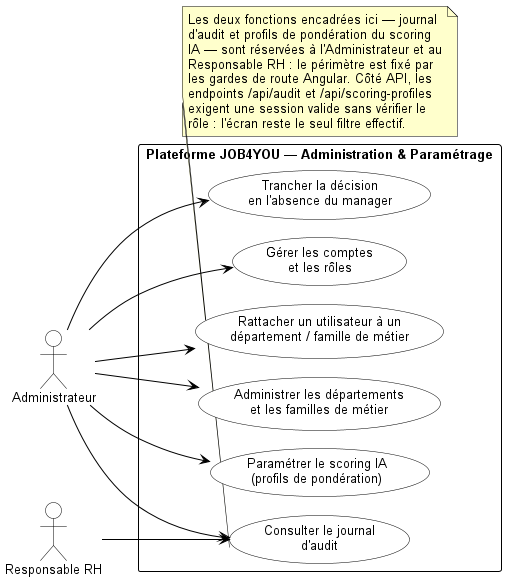
\includegraphics[width=\textwidth, height=0.80\textheight, keepaspectratio]{fig2_5}
\caption{Diagramme de cas d’utilisation — Administration \& Paramétrage}
\label{fig_2_5}
\end{figure}

\subsection{Description textuelle de quelques cas d’utilisation}
\label{sec_2_2_6}
Le tableau qui suit détaille le scénario nominal de deux cas d’utilisation représentatifs du processus métier.

% tableau 2.2
\setcounter{table}{1}
\begin{table}[!ht]
\centering
\caption{Description textuelle de deux cas d’utilisation représentatifs}
\label{tab_2_2}
\renewcommand{\arraystretch}{1.25}\footnotesize
\setlength{\tabcolsep}{4pt}%
\begin{tabular}{|P{0.097\textwidth}|P{0.311\textwidth}|P{0.538\textwidth}|}
\hline
\textbf{Élément} & \textbf{Cas d’utilisation « Postuler à une offre »} & \textbf{Cas d’utilisation « Avis manager, puis décision finale »} \\
\hline
Acteur principal & Candidat & Manager (avis), puis Responsable RH (contreseing) \\
\hline
Pré-condition & L’offre est publiée (statut ACTIVE) & Le dossier a été transmis au manager pour évaluation technique : un avis favorable (ACCEPTED) comme un refus proposé (MANAGER\_REJECTED) sont admis sur les seuls statuts TECHNICAL\_TEST, INTERVIEW et FINAL\_INTERVIEW, c’est-à-dire après le pré-filtrage téléphonique du RH. \\
\hline
Scénario nominal & Le candidat consulte l’offre, remplit le formulaire de candidature et dépose son CV. Le système enregistre la candidature, envoie un e-mail de confirmation et déclenche l’analyse IA du CV. & Le manager consulte le dossier du candidat, ses scores et ses éventuels feedbacks, puis émet un avis — favorable, ou refus proposé accompagné d’un motif. Le RH, averti par e-mail et dans sa liste de candidats, contresigne cet avis : embauche (HIRED) avec date de présentation des documents, ou refus final (REJECTED) motivé. \\
\hline
Post-condition & La candidature est créée avec le statut APPLIED, puis mise à jour automatiquement selon le score IA. & L’avis est enregistré (ACCEPTED ou MANAGER\_REJECTED) et notifié au RH ; la décision finale (HIRED ou REJECTED) n’est acquise qu’après son contreseing, seul moment où le candidat reçoit un e-mail. \\
\hline
Exception & Candidature déjà déposée pour cette offre : le système rejette la demande. & Dossier à un statut qui n’autorise pas la décision demandée — par exemple un avis favorable avant l’entretien téléphonique RH — ou refus manager sans motif : le système retourne une erreur 400. Un compte purement manager qui appelle le point d’entrée de validation finale reçoit une erreur 403. \\
\hline
\end{tabular}
\end{table}
\subsection{Diagramme de séquence système (boîte noire)}
\label{sec_2_2_7}
Le diagramme de la figure~\ref{fig_2_6} adopte une approche « boîte noire » stricte : il modélise uniquement les échanges entre l’acteur Candidat et le système JOB4YOU considéré comme un tout. Il met en évidence la requête de soumission du formulaire et le retour synchrone de confirmation (HTTP 201 Created), masquant à ce stade l’infrastructure interne et les traitements asynchrones, qui relèvent de la conception détaillée (section~\ref{sec_3_4}).

% figure 2.6
\setcounter{figure}{5}
% remise en portrait et a taille naturelle : le PNG source ne mesure que 418 x 255 px.
% Etalee sur une page paysage entiere, l'image s'imprimait a ~1,6 fois sa taille,
% donc en flou, et coutait une page pleine. A 0,70\linewidth elle imprime
% 337 pt de large (police ~9,7 pt), sans qu'aucun pixel ne soit agrandi.
\begin{figure}[!ht]
\centering
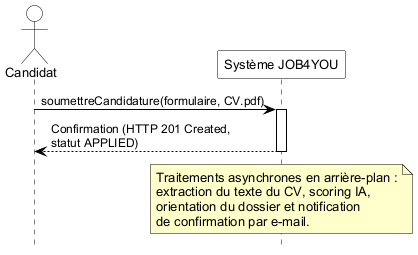
\includegraphics[width=0.70\linewidth]{fig2_6}
\caption{Diagramme de séquence système — Soumettre une candidature (boîte noire)}
\label{fig_2_6}
\end{figure}

\section{Étude technique}
\label{sec_2_3}
Les choix techniques répondent aux besoins identifiés. Spring Boot \cite{ref04,ref05} a été retenu pour la robustesse de son écosystème (Spring Security, Spring Data JPA) et la rapidité de mise en place d’API REST sécurisées. Angular \cite{ref06,ref07} impose une structure (composants, services, routage, gardes de route) adaptée à une application multi-rôles maintenue dans la durée. PostgreSQL \cite{ref08} offre un modèle relationnel solide et des garanties transactionnelles pour des données fortement liées (offres, candidatures, entretiens, feedbacks). Enfin, n8n \cite{ref09} permet de construire et de faire évoluer les workflows d’automatisation (planification, notifications, déclenchement du scoring) sans alourdir le code du back-end, tout en isolant les dépendances vis-à-vis des services externes.

\subsection{Architecture physique cible}
\label{sec_2_3_1}
La plateforme cible une architecture distribuée par couches : un front-end Angular servi au navigateur, un back-end Spring Boot exposant des API REST sécurisées, une base PostgreSQL (SGBD) et une couche d’automatisation n8n chargée de la planification des entretiens (Google Calendar \cite{ref10}) et de l’essentiel des notifications (SMTP) ; le back-end envoie toutefois ses propres courriels, via JavaMailSender, pour la réinitialisation du mot de passe et les rappels d’entretien. Il appelle aussi directement l’API de Cohere \cite{ref11} (scoring IA) et l’API OpenRouter \cite{ref12} (assistant conversationnel). Cette organisation physique est détaillée au chapitre 3 (figures~\ref{fig_3_10} et \ref{fig_3_11}) ; le tableau~\ref{tab_2_3} précise le rôle de chaque agent.

% tableau 2.3
\setcounter{table}{2}
\begin{table}[!ht]
\centering
\caption{Rôle des agents d’automatisation n8n}
\label{tab_2_3}
\renewcommand{\arraystretch}{1.25}\footnotesize
\setlength{\tabcolsep}{4pt}%
\begin{tabular}{|P{0.166\textwidth}|P{0.236\textwidth}|P{0.545\textwidth}|}
\hline
\textbf{Agent} & \textbf{Déclencheur} & \textbf{Rôle et traitement} \\
\hline
Agent 1 — « CV Parser + Score IA + Email Candidat » (scoring IA) & Webhook déclenché à la création d’une candidature (statut APPLIED) & Extrait le texte du CV puis rappelle le back-end (POST \path{/api/candidates/\{id\}/ai-score/recompute}). C’est le back-end, via son client CohereClient, qui interroge l’API de Cohere, calcule le score et le persiste ; le statut bascule ensuite vers CV\_REVIEWED ou AUTO\_REJECTED selon le seuil. \\
\hline
Agent 2 — « Planification entretien + Email participants » (Google Meet et convocations) & Webhook déclenché à la planification d’un entretien & Crée réellement l’événement Google Calendar, génère le lien Google Meet correspondant, ajoute les participants et envoie la convocation au candidat comme la confirmation à l’intervieweur. \\
\hline
Agent 3 — « RH vers Manager (dossier validé) » (notification du manager désigné) & Webhooks déclenchés à l’entrée en évaluation technique (TECHNICAL\_TEST), au rejet automatique et au retrait d’une candidature & Notifie le manager désigné par le RH, résolu et gelé sur le dossier par le back-end (Manager\-Routing\-Service), sans dupliquer l’e-mail candidat ; les e-mails de décision — avis transmis au RH, convocation ou refus final adressé au candidat — sont émis par le back-end via NotificationService. \\
\hline
\end{tabular}
\end{table}
\subsection{Côté client — Angular}
\label{sec_2_3_2}
J’ai développé le front-end sous forme de SPA (Single Page Application) avec Angular, en architecture par composants autonomes (« standalone components »), organisée en pages publiques (accueil, offres d’emploi, candidature en ligne), pages d’administration (candidats, entretiens, feedbacks, offres, utilisateurs, tableau Kanban, tableau de bord) et services partagés qui assurent la communication avec l’API REST du back-end. Bootstrap prend en charge la mise en forme des interfaces.

\subsection{Côté serveur — Spring Boot}
\label{sec_2_3_3}
Côté serveur, j’ai développé le back-end en Java avec Spring Boot 3, selon une architecture en couches classique : contrôleurs REST, services métier, repositories Spring Data JPA et entités JPA (mapping objet-relationnel, ORM, assuré par Hibernate) mappées sur la base PostgreSQL. Cette organisation garde les responsabilités bien séparées et facilite les évolutions futures.

\subsection{La sécurité — Spring Security et JWT}
\label{sec_2_3_4}
L’accès à la plateforme repose sur Spring Security \cite{ref13}, couplé à une authentification par jeton JWT (JSON Web Token). À la connexion, le serveur génère un jeton signé portant l’identité et les rôles de l’utilisateur ; ce jeton est ensuite transmis dans l’en-tête de chaque requête, ce qui authentifie l’utilisateur sans nécessiter d’état de session côté serveur. Chaque point d’entrée de l’API est protégé via l’annotation @PreAuthorize, garantissant que seuls les rôles autorisés (Administrateur, RH, Manager) accèdent à une ressource donnée.

\section{Conclusion}
\label{sec_2_4}
Acteurs, besoins et architecture technique étant désormais clairement identifiés, une question s’est imposée : comment traduire tout cela en un modèle concret, capable de guider le développement ? C’est ce que j’aborde dans le chapitre suivant, consacré à la conception.
